\documentclass{rapport}
\usepackage[utf8]{inputenc}

\usepackage{pifont} % Pour les symboles appelés par la macro \ding
\usepackage{url} % Comme son nom l'indique, pour les url...

\usetikzlibrary{positioning} % Bibliothèque tikz pour positionner des nœuds relativement à d'autres

\usepackage[colorlinks, citecolor=red!60!green, linkcolor=blue!60!green, urlcolor=magenta]{hyperref} % Pour que les liens soient cliquables. Les options permettent de mettre les liens en couleur.

\usepackage{algorithm}
\usepackage{algo}
\usepackage{colorationSyntaxique}
\usepackage{amsmath}
\usepackage{diagbox}
\usepackage{graphicx}
\usepackage{listings}
\lstset{                  % Specify language
    basicstyle=\ttfamily\small,     % Code font and size
    keywordstyle=\color{blue},      % Color for keywords
    commentstyle=\color{gray},      % Color for comments
    stringstyle=\color{red},        % Color for strings
    numbers=left,                   % Add line numbers
    numberstyle=\tiny\color{gray},  % Style for line numbers
    % frame=single,                   % Add a border around code
    breaklines=true,                % Line wrapping
    % backgroundcolor=\color{gray!10} % Light gray background
}

\setlength{\intextsep}{0pt} 
\setlength{\textfloatsep}{0pt}
\setlength{\parskip}{0pt} 
\setlength{\parindent}{15pt}
% Pour un rapport en français 
\usepackage[french]{babel} % Commenter pour un rapport en anglais
\renewcommand\bibsection{\section*{Bibliographie}} % Commenter pour un rapport en anglais

% \englishTitlePage % Décommenter pour une page de titre en anglais

\pagestyle{fancy}
\renewcommand{\sectionmark}[1]{\markboth{\thesection.\ #1}{}}
\fancyfoot{}

\fancyhead[LE]{\textsl{\leftmark}}
\fancyhead[RE, LO]{\textbf{\thepage}}
\fancyhead[RO]{\textsl{\rightmark}}

\def\Latex{\LaTeX\xspace}
\def\etc{\textit{etc.}\xspace}



\title{Mesure et analyse de la consommation d’énergie électrique des
programmes}
\author{Mehdi Mansour}
\supervisor{Professeur Sid Touati}
\date{Premier semestre de l'année 2024-2025}

%\universityname{Université Côte d'Azur} % Nom de l'université.
\type{TP4} % Type de document
% \formation{Master Informatique} % Nom de la formation

% Retrouver les autres options possibles dans le document rapport.pdf

\begin{document}

  \maketitle

  \begin{abstract}
    Ce rapport a pour objectif de détailler les différents résultats obtenus lors de ce TP4 disponible dans l'archive.
    %\newcommand{\ppc}{programmation par contraintes\xspace}
\subsection*{Architecture utilisée pour ce TP}
     \noindent
     Architecture : x86\_64
     \newline
      \noindent
     nom CPU :	Intel(R) Core(TM) i7-10700F CPU @ 2.90GHz
     \newline
     Type de CPU :	Intel Cometlake processor
     \newline
     CPU stepping:	5
     \newline
     Hyperthreading activé
     \newline
     Sockets:		1
     \newline
     Cœurs par socket:	8
     \newline
     Threads par cœurs:	2
     \newline
     Socket 0:		( 0 8 1 9 2 10 3 11 4 12 5 13 6 14 7 15 )
     \newline
     \newline
     NUMA :
     \newline \indent
         Nœud(s) NUMA : 1
          \newline \indent
         Nœud NUMA 0 de processeur(s) : 0-15
     \newline
     Processeurs:		( 0 8 1 9 2 10 3 11 4 12 5 13 6 14 7 15 )
     \newline
     Distances:		10
     \newline
     RAM disponible:		21746.9 MB
     \newline
     RAM Total :		31991.4 MB
 \subsection*{Environnement logiciel}
 Version et distribution Linux : Debian 12

\subsection*{Topologie du PC}
    \begin{table}[h!]
    \centering
    \begin{tabular}{|c|c|c|c|c|c|c|c|c|}
        \hline
        \multicolumn{9}{|c|}{Topologie graphique} \\
        \hline
        Core & \enspace0\enspace\enspace8 &\enspace1\enspace\enspace9 &\enspace2\enspace\enspace10 &\enspace3\enspace\enspace11 &\enspace4\enspace\enspace12 &\enspace5\enspace\enspace13 &\enspace6\enspace\enspace14 &\enspace7\enspace\enspace15\\
        \hline
        Cache L1& \enspace32 kB &\enspace32 kB &\enspace32 kB &\enspace32 kB &\enspace32 kB&\enspace32 kB&\enspace32 kB&\enspace32 kB\\
        \hline
        Cache L2 & 256 kB & 256 kB & 256 kB & 256 kB & 256 kB& 256 kB& 256 kB& 256 kB\\
        \hline
        Cache L3 & \multicolumn{8}{|c|}{16 MB} \\
        \hline
    \end{tabular}
    %\caption{Les différents niveaux de cache par cœur}
    \label{tab:graph_characteristics}
    \end{table}
  
  \clearpage
  \tableofcontents

  \clearpage
%«»

  \part{Introduction}
    L'objectif de ce TP est d'étudier la consommation d'énergie électrique des programmes. Pour cela, nous utiliserons l'outil \href{https://github.com/labDomolandes/ecofloc}{EcoFloc}, qui capture la consommation d'énergie d'un programme dans un temps donné grâce à son pid. Notre objectif est donc de calculer la consommation de trois programmes (disponibles dans l'archive) : 
    \begin{itemize}
        \item «cpu.c»
        \item «memory.c»
        \item «rw.c»
    \end{itemize}
    Pour récupérer des données, il faut suivre une méthode fastidieuse. Il faut deux terminaux :
    \begin{itemize}
        \item l'un pour exécuter le programme et récupérer son pid
        \item l'autre pour effectuer les commandes EcoFloc 
    \end{itemize}
    Pour faciliter notre travail, nous allons utiliser un script nommé «exec.sh» qui réalisera cette méthode à notre place.
    Pour visualiser nos résultats nous utiliserons enfin \textit{RStudio}, un IDE pour le langage R, permettant de visualiser graphiquement des données que nous récolterons au fur-et-à-mesure du TP.

  %\pageblanche
  \clearpage
  %--------------------------------------Part II-----------------------------------------------------------
  \part{Installation et prise en main}
    Cette partie est sans doute la plus difficile de ce TP. Il faut suivre en détail les indications d'installation puis tester l'outil. Dans notre cas, pour effectuer nos calculs, il faut obligatoirement lancer la commande suivantes dans le répertoire \textit{/opt/ecofloc} ce qui n'est pas spécifié lors de l'installation, probablement à cause d'une erreur lors de l'installation :
    \begin{lstlisting}
./ecofloc-cpu.out -i 1000 -t 10 -p 55334

exemple de resultat obtenu  : 
*****************************
/ECOFLOC_CPU_PID_55334
*****************************
Average Power : 0.38 Watts
Total Energy : 3.41 Joules
*****************************
\end{lstlisting}
\newline \indent
Pour que EcoFloc récupère bien les données il faut que notre programme ne se finisse pas trop vite, ce qui était le cas au début. 
\newline\newline\indent
Nous avons donc opté, dans un premier temps, pour une boucle infinie, mais cela posait problème car nous ne pouvions pas exécuter un script avec une boucle infinie (ce qui empèche de passer d'une exécution à une autre). 
\newline\newline\indent
Nous avons dans un second temps, bloqué l'exécution avec un \textit{scanf()} pour récupérer le pid du programme sans entrer dans la boucle et ainsi lancer la commande d'EcoFloc pour récupérer nos données. Cette méthode n'était pas possible à généraliser avec un script car la boucle infinie ne peut se terminer que si on l'interrompt manuellement, ce qui interrompt également le script. 
\newline\newline\indent
Nous avons donc finalement opté pour l'ajout d'une horloge, grâce à la librairie \textit{time.h}, pour que la boucle se termine au bout d'un certain temps. Nous n'avions plus besoin du \textit{scanf()}, car grâce à l'horloge et au script «exec.sh», nous pouvions exécuter le fichier binaire, récupérer le pid, lancer la commande d'EcoFloc et écrire les résultats dans un fichier csv pour être interprété par RStudio. \newline \underline{Exemple} :  
\begin{lstlisting}
./fichier_binaire 10, la boucle durera 10sec
\end{lstlisting}
Pour généraliser cela, notre script pouvant prendre 2 arguments (le temps (obligatoire) et le nombre de répétition (par défaut à 1)) va exécuter cette méthode avec tous les fichiers binaires. \newline \underline{Exemple} :
\begin{lstlisting}
./exec.sh 10 2 
\end{lstlisting}
EcoFloc va récupérer pour chaque fichier binaire, la consommation d'énergie sur les 10 prochaines secondes et le tout 2 fois. Pour éviter d'être trop rapide, on rajoute 2 secondes au temps passé en argument. Ce qui veut dire que pour chaque exécution, la boucle du programme durera 2 secondes de plus que le temps de calcul d'EcoFloc pour lui permettre de récupérer les données à temps.

\clearpage
\part{Micro-benchmarks CPU-bound}
    Dans cette partie nous allons appliquer la méthode décrite plus haut au programme «cpu.c». Nous allons calculer la consommation de ce programme pour différentes options d'optimisation et différents compilateurs (ici \textit{gcc} et \textit{icx}). Pour cela, nous compilons notre programme grâce au script «compiler.sh».
    \section{Capture des données sur 10 secondes}
    Nous allons dans un premier temps exécuter notre script «exec.sh» 2 fois pour 10 secondes avec la commande :
    \begin{lstlisting}
./exec.sh 10 2 
\end{lstlisting}
Nos résultats sont stockés dans «res10s.csv» puis traités dans \textit{RStudio}. Nous obtenons les graphiques suivants :

\begin{figure}[H]
    \centering
    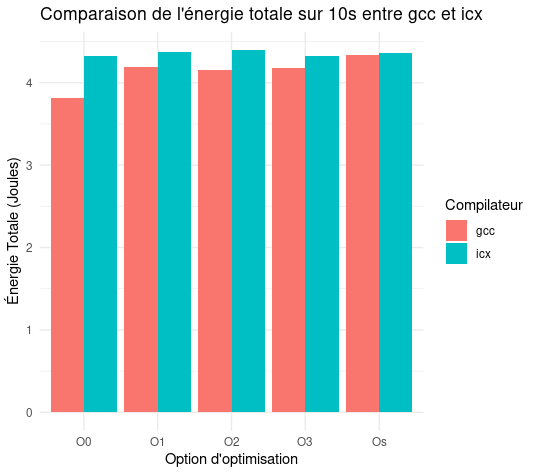
\includegraphics[width=0.5\textwidth]{../cpu/Energie10s.png}
    %\caption{}
    %\label{fig:compact}
\end{figure}

\begin{figure}[H]
    \centering
    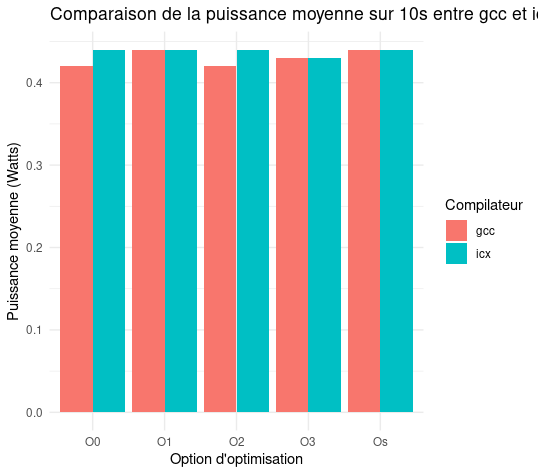
\includegraphics[width=0.5\textwidth]{../cpu/Puissance10s.png}
    %\caption{}
    %\label{fig:compact}
\end{figure}

On remarque que \textit{gcc} consomme moins d'énergie que \textit{icx}. On remarque également que la consommation électrique augmente en fonction de l'option d'optimisation pour \textit{gcc}. 
\newline Pour icx cette consommation est stable. Pour la puissance moyenne, cela varie mais globalement \textit{gcc} utilie moins de puissance électrique que \textit{icx}.
    \section{Capture des données sur 60 secondes}
    Nous allons dans un premier temps exécuter notre script «exec.sh» 1 fois pour 60 secondes avec la commande :
    \begin{lstlisting}
./exec.sh 60
\end{lstlisting}
Nos résultats sont stockés dans «res60s.csv» puis traités dans \textit{RStudio}. Nous obtenons les graphiques suivants :

\begin{figure}[H]
    \centering
    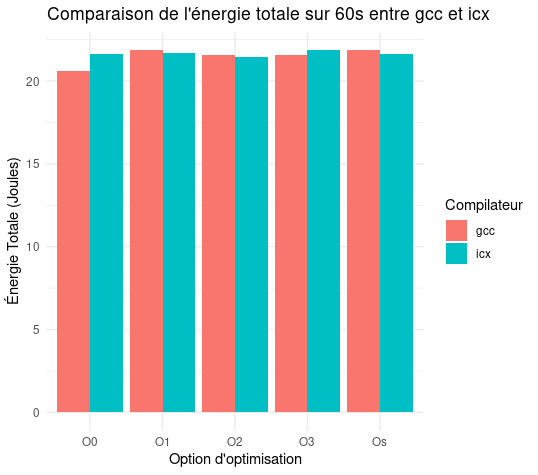
\includegraphics[width=0.5\textwidth]{../cpu/Energie60s.png}
    %\caption{}
    %\label{fig:compact}
\end{figure}

\begin{figure}[H]
    \centering
    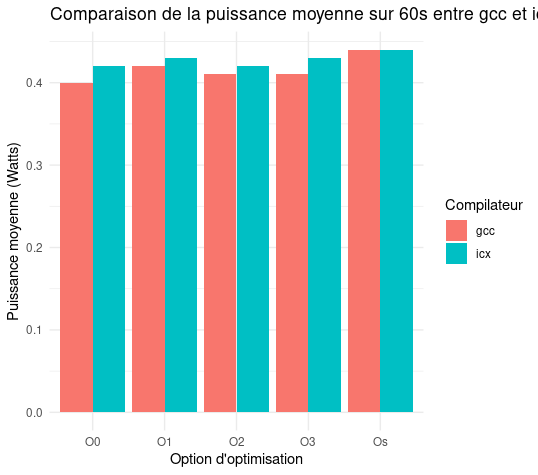
\includegraphics[width=0.5\textwidth]{../cpu/Puissance60s.png}
    %\caption{}
    %\label{fig:compact}
\end{figure}

On remarque que \textit{gcc} consomme plus d'énergie de manière général que \textit{icx} (consomme plus que \textit{icx} en O1, O2, Os). Cette consommation augmente légèrement en fonction des options. Pour la puissance électrique, comme pour 10 secondes, \textit{gcc} consomme moins de puissance. 

\clearpage
\part{Micro-benchmarks Memory-bound}\setcounter{section}{0}
    Dans cette partie nous allons appliquer la méthode décrite plus haut au programme «cpu.c». Nous allons calculer la consommation de ce programme pour différentes options d'optimisation et différents compilateurs (ici \textit{gcc} et \textit{icx}). Pour cela, nous compilons notre programme grâce au script «compiler.sh».
    \section{Capture des données sur 10 secondes}
    Nous allons dans un premier temps exécuter notre script «exec.sh» 2 fois pour 10 secondes avec la commande :
    \begin{lstlisting}
./exec.sh 10 2 
\end{lstlisting}
Nos résultats sont stockés dans «res10s.csv» puis traités dans \textit{RStudio}. Nous obtenons les graphiques suivants :

\begin{figure}[H]
    \centering
    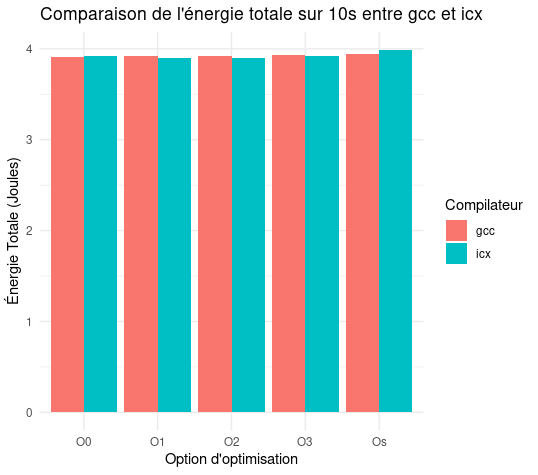
\includegraphics[width=0.5\textwidth]{../memory/Energie10s.png}
    %\caption{}
    %\label{fig:compact}
\end{figure}

\begin{figure}[H]
    \centering
    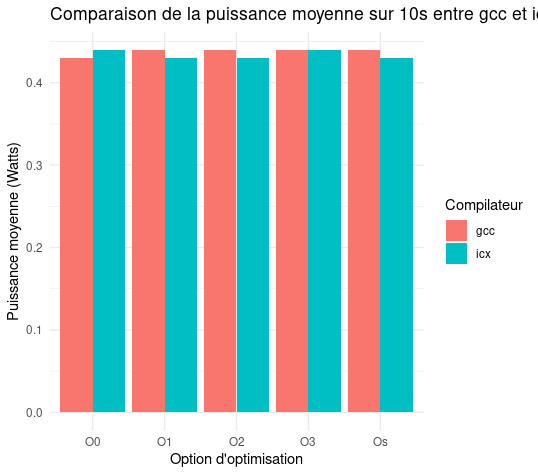
\includegraphics[width=0.5\textwidth]{../memory/Puissance10s.png}
    %\caption{}
    %\label{fig:compact}
\end{figure}

On remarque que \textit{icx} consomme moins d'énergie que \textit{gcc} pour les options O1, O2 et O3. On a une consommation d'énergie stable quel que soit l'option pour les deux compilateurs. Pour la puissance électrique, \textit{gcc} en consomme plus qu'\textit{icx} pour les options O1, O2, Os.

    \section{Capture des données sur 60 secondes}
Nous allons dans un premier temps exécuter notre script «exec.sh» 1 fois pour 60 secondes avec la commande :
    \begin{lstlisting}
./exec.sh 60
\end{lstlisting}
Nos résultats sont stockés dans «res60s.csv» puis traités dans \textit{RStudio}. Nous obtenons les graphiques suivants :

\begin{figure}[H]
    \centering
    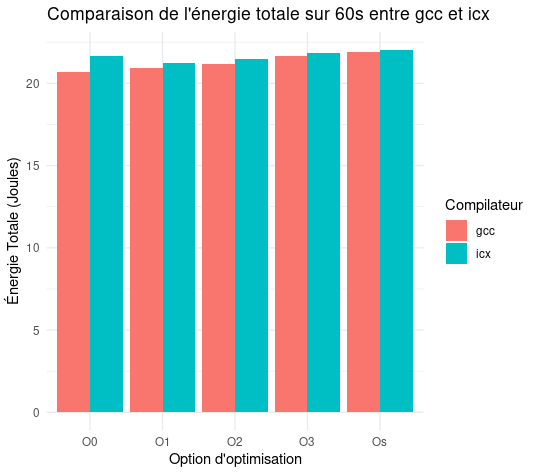
\includegraphics[width=0.5\textwidth]{../memory/Energie60s.png}
    %\caption{}
    %\label{fig:compact}
\end{figure}

\begin{figure}[H]
    \centering
    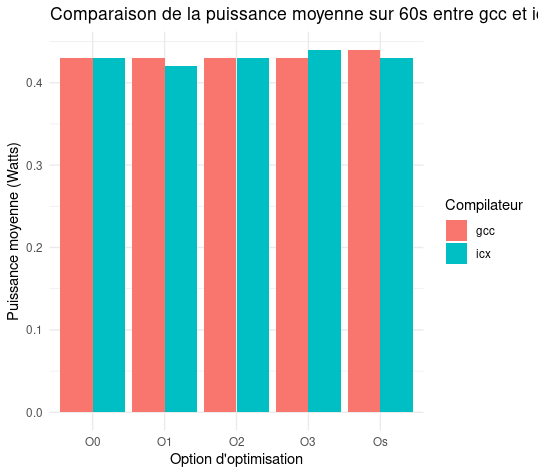
\includegraphics[width=0.5\textwidth]{../memory/Puissance60s.png}
    %\caption{}
    %\label{fig:compact}
\end{figure}

On remarque que pour 60 secondes, \textit{gcc} consomme moins d'énergie que \textit{icx} pour chaque option. On constate que la consommation d'énergie augmente en fonction des options pour les deux compilateurs. En ce qui concerne la puissance électrique, les deux se valent (\textit{icx} légèrement mieux).

\clearpage
\part{Micro-benchmarks avec des appels système}\setcounter{section}{0}
    Dans cette partie nous allons appliquer la méthode décrite plus haut au programme «cpu.c». Nous allons calculer la consommation de ce programme pour différentes options d'optimisation et différents compilateurs (ici \textit{gcc} et \textit{icx}). Pour cela, nous compilons notre programme grâce au script «compiler.sh».
    \section{Capture des données sur 10 secondes}
    Nous allons dans un premier temps exécuter notre script «exec.sh» 2 fois pour 10 secondes avec la commande :
    \begin{lstlisting}
./exec.sh 10 2 
\end{lstlisting}
Nos résultats sont stockés dans «res10s.csv» puis traités dans \textit{RStudio}. Nous obtenons les graphiques suivants :

\begin{figure}[H]
    \centering
    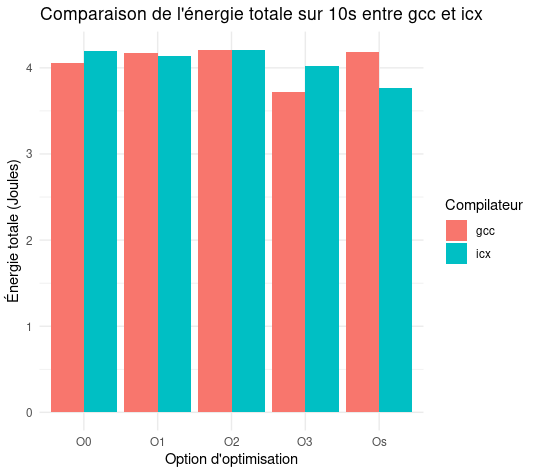
\includegraphics[width=0.5\textwidth]{../af/Energie10s.png}
    %\caption{}
    %\label{fig:compact}
\end{figure}

\begin{figure}[H]
    \centering
    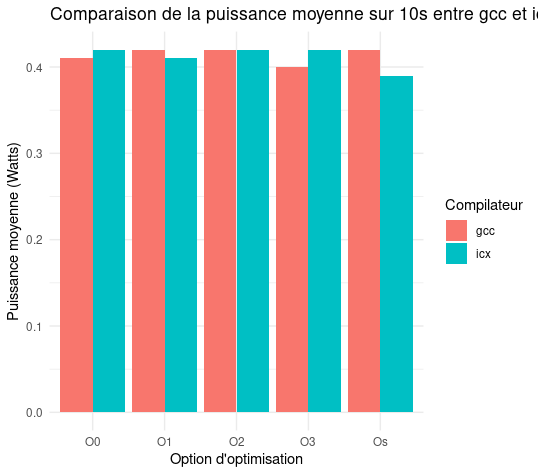
\includegraphics[width=0.5\textwidth]{../af/Puissance10s.png}
    %\caption{}
    %\label{fig:compact}
\end{figure}

On remarque que les compilateurs se valent pour la consommation d'énergie. La consommation d'énergie est rélativement stable quel que soit l'option. En ce qui concerne la puissance électrique, les deux compilateurs se valent également.

    \section{Capture des données sur 60 secondes}
    Nous allons dans un premier temps exécuter notre script «exec.sh» 1 fois pour 60 secondes avec la commande :
    \begin{lstlisting}
./exec.sh 60
\end{lstlisting}
Nos résultats sont stockés dans «res60s.csv» puis traités dans \textit{RStudio}. Nous obtenons les graphiques suivants :

\begin{figure}[H]
    \centering
    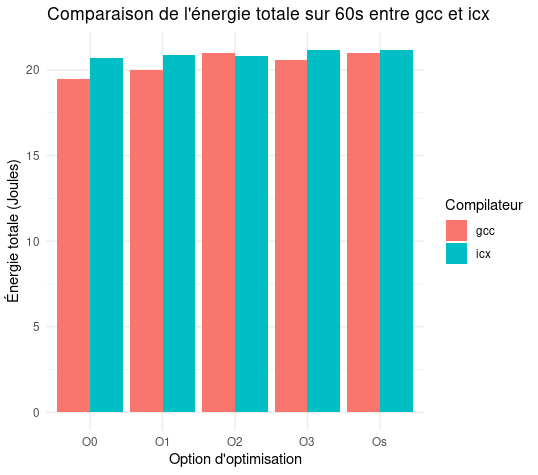
\includegraphics[width=0.5\textwidth]{../af/Energie60s.png}
    %\caption{}
    %\label{fig:compact}
\end{figure}

\begin{figure}[H]
    \centering
    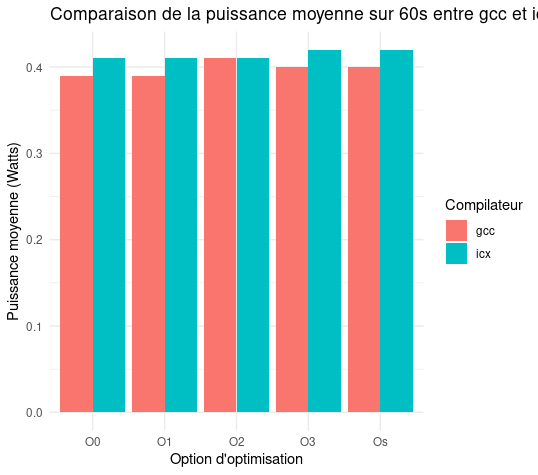
\includegraphics[width=0.5\textwidth]{../af/Puissance60s.png}
    %\caption{}
    %\label{fig:compact}
\end{figure}

On remarque que \textit{gcc} consomme moins d'énergie que \textit{icx}. Il consomme également moins de puissance électrique que \textit{icx}. La consommation d'énergie est rélativement stable quel que soit l'option pour les deux compilateurs.

\clearpage
\part{Conclusion}
\indent
Dans le cadre de ce TP, nous avons étudié la consommation d'énergie électrique des programmes. Nous avons remarqué que plus l'exécution est longue et plus la consommation augmente.
Les résultats obtenus lors de ce TP doivent être interprétés avec précaution, car la consommation peut varier d'une exécution de script à l'autre en raison de la présence d'autres processus en cours. Il ne faut pas négliger cela. Ces resultats donnent malgré tout un ordre d'idée de la consommation d'énergie électrique d'un programme.
\newline
En ce qui concerne EcoFloc, c'est un outil utile mais qui devient fastidieux s'il est utilisé manuellement pour chaque programme. Dans notre cas, l'utilisation d'un script était nécessaire.
\end{document}
